\documentclass{article}
\usepackage{listings}
\usepackage{graphicx}

\usepackage{xcolor}

\definecolor{codegreen}{rgb}{0,0.6,0}
\definecolor{codegray}{rgb}{0.5,0.5,0.5}
\definecolor{codepurple}{rgb}{0.58,0,0.82}
\definecolor{backcolour}{rgb}{0.95,0.95,0.92}

\lstdefinestyle{mystyle}{
    backgroundcolor=\color{backcolour},   
    commentstyle=\color{codegreen},
    keywordstyle=\color{magenta},
    numberstyle=\tiny\color{codegray},
    stringstyle=\color{codepurple},
    basicstyle=\ttfamily\footnotesize,
    breakatwhitespace=false,         
    breaklines=true,                 
    captionpos=b,                    
    keepspaces=true,                 
    numbers=left,                    
    numbersep=5pt,                  
    showspaces=false,                
    showstringspaces=false,
    showtabs=false,                  
    tabsize=2
}

\lstset{style=mystyle}

\title{ChildSynth: Leveraging Synthetic Imagery for Automated Height Measurement in Malnutrition Prediction}
\author{David Berthiaume}

\begin{document}

\maketitle



\section{Introduction}

Predicting Childhood Malnutrition is a critical task in the field of public health. Malnutrition among children is still a significant public health problem in many developing countries. It is a primary cause of morbidity and mortality in children. Malnutrition is a condition that results from eating a diet in which one or more nutrients are insufficient, such that the diet causes health problems.

This paper proposes a novel approach to predict malnutrition in children using synthetic imagery. 
We leverage the power of synthetic data to help evaluate and train several deep-learning models to predict heights in children to support the prediction of malnutrition. 

Obtaining data for training deep learning models is a challenging task. The data must be labeled and annotated, which can be time-consuming and expensive. Obtaining images of children to train a model to predict malnutrition is even more challenging. These images and height measurements must be taken in a controlled environment with trained personnel to ensure high accuracy. Furthermore, this data is sensitive since it involves images of children.

To combat these challenges, a synthetic data generator, ChildSynth, has been developed to create images of children with height measurements. This synthetic data generator can create an unlimited number of images of children with varying characteristics and pixel-perfect heights. The generated synthetic data can be used to evaluate and pre-train deep learning models to predict children's height. 

\section{ChildSynth}

ChildSynth is a command-line program that uses procedural modeling and ray tracing to generate color images, depth maps, segmentation maps, keypoints, precise height measurements, and auxiliary information for synthetic children lying on a mat as viewed from different camera angles. The following example generates RGB images, depth maps, segmentation maps, and auxiliary text files with height measurements and other characteristics for $5$ different camera angles for a total of $15$ images. 

\begin{lstlisting}[language=bash]
python render_children.py --resy 512 --resx 512 --num_children 1     --output_dir ./output 
\end{lstlisting}

Figure \ref{fig:child_0} shows an example of a synthetic child generated by the above command.

\begin{figure}[]
    \centering
    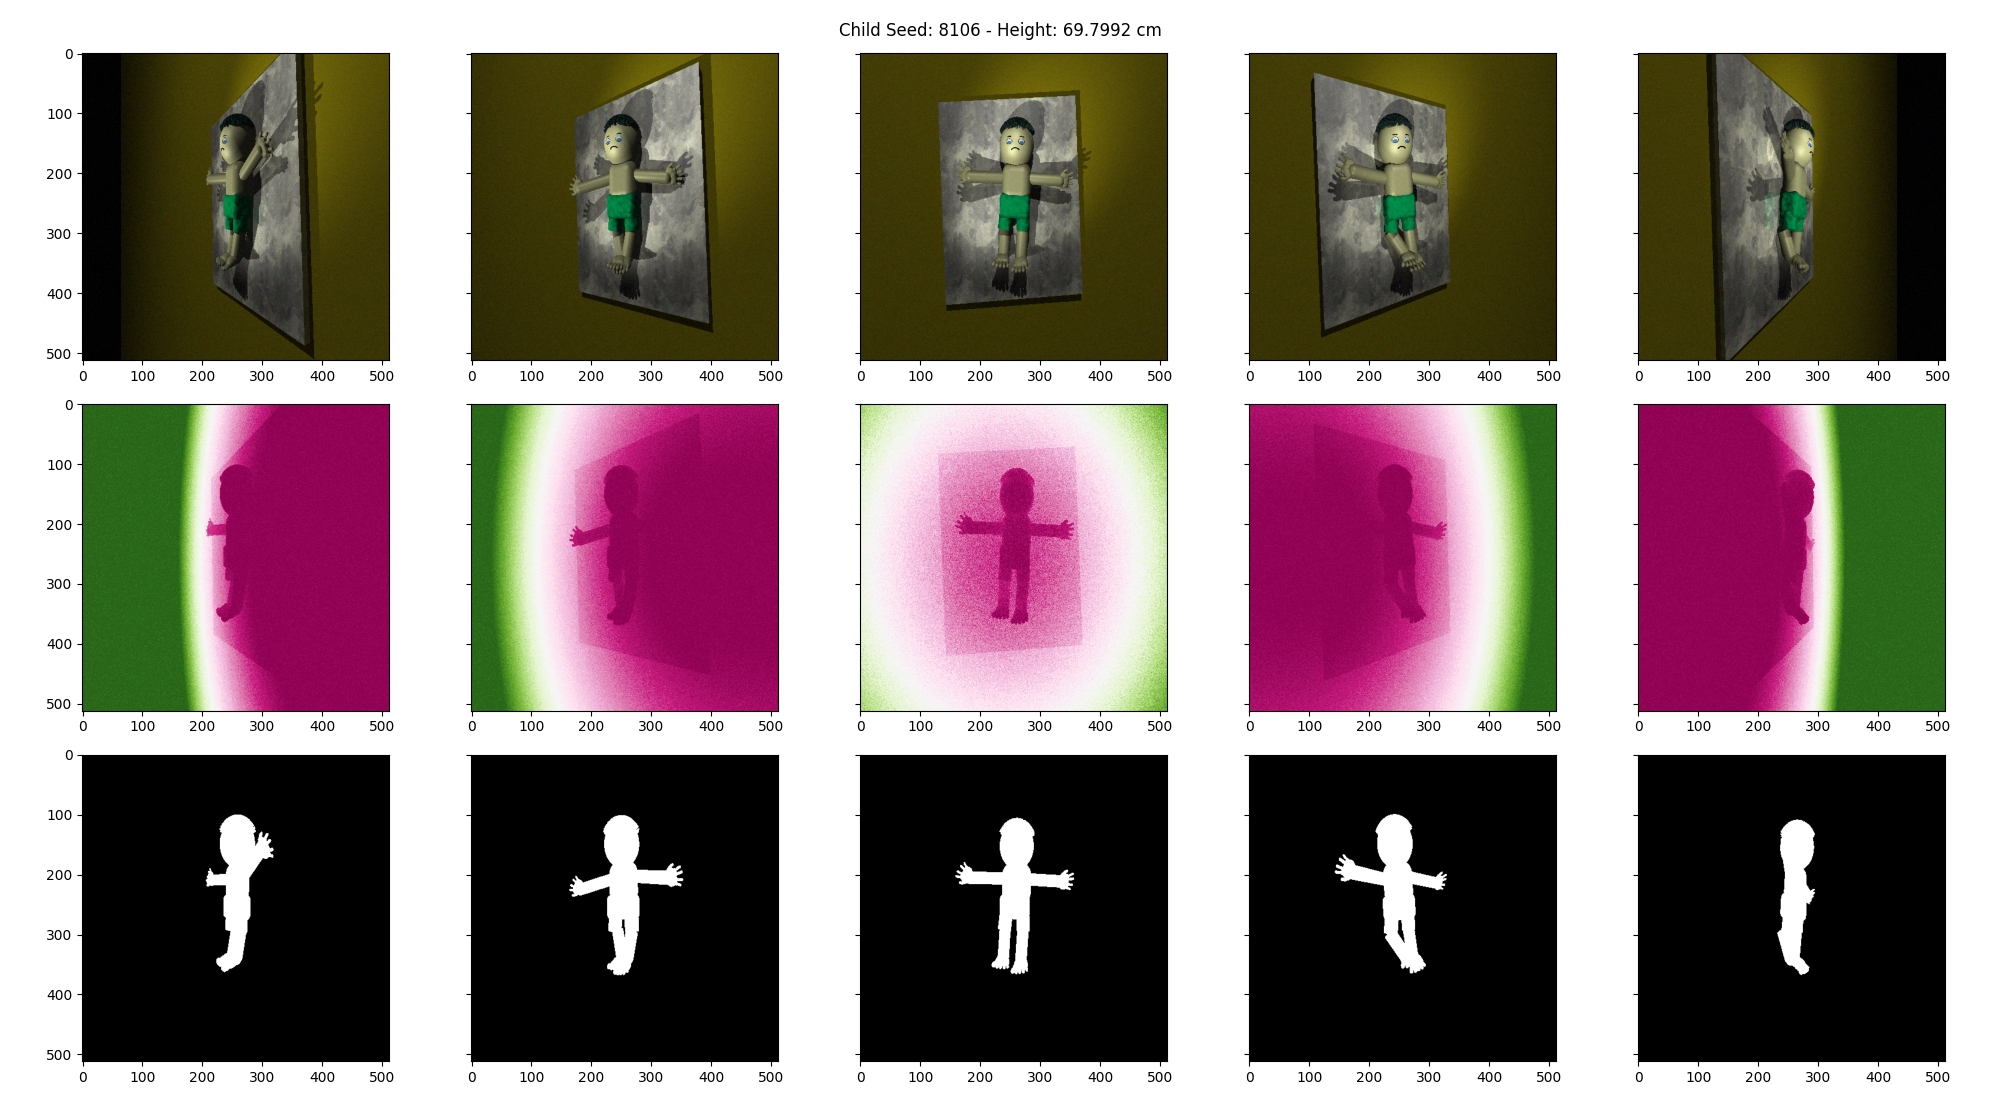
\includegraphics[width=\textwidth]{plots/child_0.png}
    \caption{Example of a synthetic child generated by ChildSynth. The upper row consists of color images, the middle row consists of depth maps, and the bottom row consists of binary segmentation maps indicating whether each pixel is part of a child or part of the background.}
    \label{fig:child_0}
\end{figure}

The goal of ChildSynth is not to generate photorealistic images but to parametrically model children with infinite variations. Every element, the length, style, density, and color of hair, the facial characteristics, the skin and mat textures, even the size of each toe, is modeled parametrically and can be individually specified or sampled from various random distributions. Elements of the scene, including camera position, lighting, and image quality, are also parametrically modeled. One can specify over $60$ different parameters to control how the children and scenes are generated.

\section{Approach}
\subsection{Rendering}

ChildSynth renders Each parametrically modeled scene using ray tracing. The geometries in the scene are composed of spheres, cylinders, cubes, rounded cubes, planes, and blobs. Blobs themselves are composed of cubes, cylinders, and spheres and allow one to parametrically create smooth shapes, such as those found in a child's body. A smooth field is created from the multiple component objects within each bloc. Each component of a blob exerts a field in the space around it, and the sum of these fields determines the shape of the blob. When the combined field strength at any point in space exceeds a given threshold value, the surface at that point becomes part of the blob. These composite objects are beneficial for creating smooth shapes parametrically with fine-grained control over the individual features of the shape. Much of the complexity of the child's body is modeled using blobs, especially for the feet and hands (see figure \ref{fig:hand_foot}). 

\begin{figure}[htbp]
    \centering
    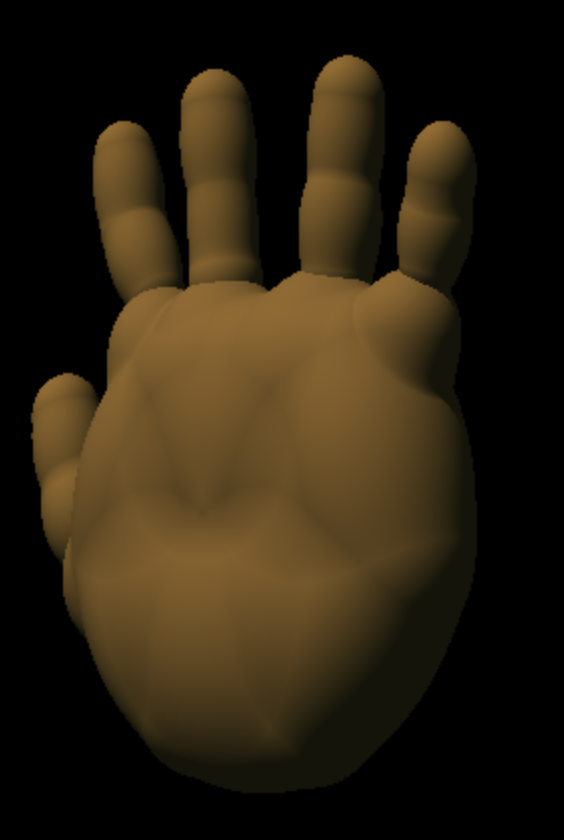
\includegraphics[height=4cm]{plots/hand.png}
    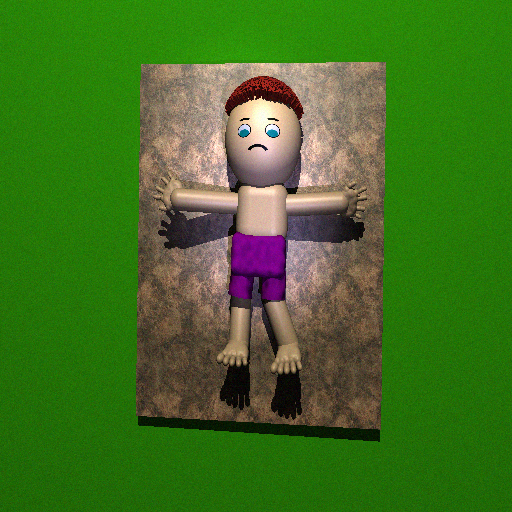
\includegraphics[height=4cm]{plots/child_000000_rgb_090.png}
    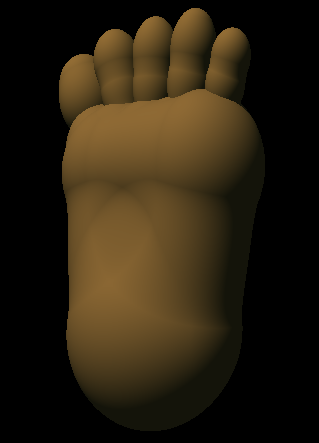
\includegraphics[height=4cm]{plots/foot.png}
    \caption{Hands and feet are rendered using blobs that consist of a complex arrangement of parametric spheres and cylinders. The strength and shape of each sphere and cylinder can be individually controlled to create a wide variety of shapes from the resulting field.}
    \label{fig:hand_foot}
\end{figure}

Each child is rendered from multiple view angles to provide a variety of perspectives. The camera is placed at different positions above the child to capture the child's body from multiple positions. By default, $5$ different camera angles are used to render each child, from $30$ to $150$ degrees, in increments of $30$ degrees, with $90$ degrees being directly above the child, and $30$ and $150$ degrees being to the left and right of the child respectively. These multiple views allow one to predict the child's height with computer vision.

ChildSynth renders a depth image corresponding to each color image by storing the distance from the camera to the scene. The depth image and the color imagery are precisely coregistered.

Finally, ChildSynth renders a binary segmentation map for each child. The segmentation map is a binary image where each pixel is either part of the child or the background. Along with the color and depth images, the segmentation map is helpful for training deep-learning models to predict the child's height.


\subsection{Modeling}

\subsubsection{Parameters}

ChildSynth can render millions of synthetic children, with no two being identical.  It accomplishes this by sampling over $60$ parameters from various probability distributions. For example, an optional spotlight may be placed around the child as a light source. The position of this spotlight is sampled from several normal distributions, with the light being most likely placed near the child. The color of this light source is sampled from three uniform distributions, one for each of the red, green, and blue intensities. 



\bibliographystyle{unsrt}
\bibliography{references}


\end{document}